\subsection{Panorama bibliométrico da literatura}\label{sec:bibliometria}

Para dimensionar o campo e orientar a seleção das referências, realizou-se um levantamento bibliométrico na base Scopus, processado com o pacote bibliometrix \citep{AriaCuccurullo2017}, em formato inspirado na abertura de \citet{Baker2022}. A busca, feita em 22 de outubro de 2026 nos títulos, resumos e palavras-chave, usou a expressão em inglês (\textit{``flypaper effect'' OR ``fiscal illusion'' OR ``intergovernmental transfer*'' OR ``intergovernmental grant*''}) AND (\textit{municipal* OR ``local government*'' OR subnational}) e foi restrita a artigos de periódicos publicados entre 2016 e 2026. Termos como \textit{fiscal transfers}, \textit{revenue sharing} e \textit{equalization} não foram incluídos; o conjunto recuperado é, portanto, uma amostra da literatura sobre transferências a governos locais, não o seu universo.

A busca retornou 327 artigos, dos quais 54 (16,5\%) tratam especificamente de efeito \textit{flypaper} ou de ilusão fiscal, critério aplicado aos títulos, resumos e palavras-chave (Tabela~\ref{tab:bibliometria} e Figura~\ref{fig:producao}). Considerados apenas os anos completos, a produção subiu de 23 artigos por ano em 2016--2019 para 32 em 2020--2022 e ficou em 29 em 2023--2025; somados, os períodos têm 92, 97 e 138 artigos, este último com 2026 incompleto. Os artigos específicos somam 15, 20 e 19 nesses períodos, ou 16,3\%, 20,6\% e 13,8\% do total. Com contagens tão pequenas, a variação dessas participações não permite afirmar uma mudança de agenda; indica apenas que os dois conceitos ocupam uma fatia estável e minoritária de uma literatura que cresceu até 2022 e depois se estabilizou.

A distribuição por periódico mostra onde esses conceitos circulam. Os títulos que mais publicam pertencem às finanças públicas e à economia política, com destaque para \textit{Local Government Studies} e \textit{Public Finance Review}, com 11 artigos cada. Em \textit{Local Government Studies} e \textit{Lex Localis}, cerca de metade dos artigos trata de \textit{flypaper} ou de ilusão fiscal; no \textit{European Journal of Political Economy}, nenhum dos dez artigos emprega esses termos, embora alguns tratem do fenômeno, como o de \citet{Shani2023}. Os demais 247 artigos (75,5\%) dispersam-se por outros periódicos. Essa base, complementada por estudos brasileiros não indexados na Scopus e por clássicos indispensáveis, forneceu o núcleo das referências discutidas a seguir.

\IfFileExists{tabelas/tabela1_bibliometria.tex}{\begin{table}[H]
\centering\footnotesize\setlength{\tabcolsep}{5pt}
\caption{Uso dos conceitos de efeito \textit{flypaper} e ilusão fiscal na literatura sobre transferências a governos locais, por periódico (2016--2026)}
\label{tab:bibliometria}
\begin{threeparttable}
\begin{tabular}{lccc}
\toprule
 & (1) & (2) & (3) \\
 & Transferências a & \textit{Flypaper} ou & (2)/(1) \\
Periódico & governos locais & ilusão fiscal & (\%) \\
\midrule
Local Government Studies & 11 & 6 & 54,5\% \\
Public Finance Review & 11 & 3 & 27,3\% \\
European Journal of Political Economy & 10 & 0 & 0,0\% \\
International Tax and Public Finance & 10 & 1 & 10,0\% \\
Public Choice & 8 & 2 & 25,0\% \\
Public Budgeting and Finance & 7 & 1 & 14,3\% \\
Lex Localis & 6 & 3 & 50,0\% \\
Regional Studies & 6 & 0 & 0,0\% \\
World Development & 6 & 0 & 0,0\% \\
Regional Science and Urban Economics & 5 & 1 & 20,0\% \\
Demais periódicos & 247 & 37 & 15,0\% \\
\midrule
Total & 327 & 54 & 16,5\% \\
\bottomrule
\end{tabular}
\begin{tablenotes}[flushleft]\footnotesize
\item Nota: A tabela resume o número de artigos publicados em periódicos científicos entre 2016 e 2026 sobre transferências intergovernamentais a governos locais. A busca foi realizada em 22/10/2026 na base Scopus, nos campos título, resumo e palavras-chave, com a expressão: ("flypaper effect" OR "fiscal illusion" OR "intergovernmental transfer*" OR "intergovernmental grant*") AND (municipal* OR "local government*" OR subnational), restrita a artigos de periódico publicados entre 2016 e 2026. A busca retornou 327 artigos. A coluna (1) apresenta todos os artigos; a coluna (2), os que tratam especificamente de efeito flypaper ou de ilusão fiscal (termos presentes no título, no resumo ou nas palavras-chave; artigos que tratam do fenômeno sem usar esses termos ficam apenas na coluna 1); a coluna (3), a participação de (2) em (1). As linhas listam os dez periódicos com mais artigos; os demais estão agregados. Os dados de 2026 são parciais (artigos indexados até a data da busca). Processamento: pacote bibliometrix (Aria e Cuccurullo, 2017) no R.
\end{tablenotes}
\end{threeparttable}
\end{table}
}{}

\IfFileExists{figuras/figura_producao_anual.png}{%
\begin{figure}[H]
  \centering
  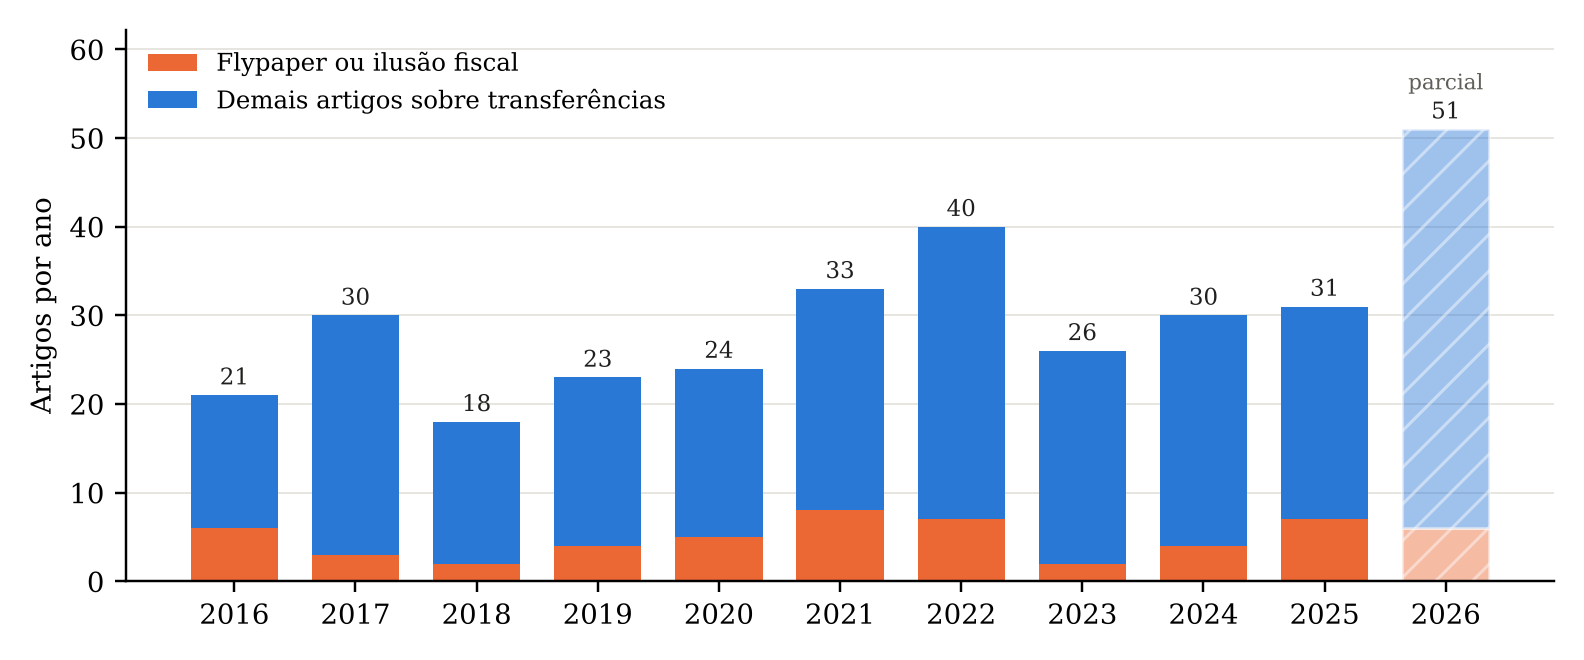
\includegraphics[width=0.9\textwidth]{figuras/figura_producao_anual.png}
  \caption{Produção anual de artigos recuperados pela busca (2016--2026): total e artigos sobre efeito \textit{flypaper} ou ilusão fiscal}
  \label{fig:producao}
  \fonte{elaboração própria a partir da base Scopus (busca em 22/10/2026), com a contagem do bibliometrix \citep{AriaCuccurullo2017}. Barras hachuradas: 2026, ano parcial.}
\end{figure}}{}
